\chapter{Preface}
\lipsum[1]

Note that the theory on machine learning and quantum computing, in addition to parts of the introduction, are based the preparatory project report~\autocite{sjo2022}, and in the case of \cref{sec:nn,sec:qstates,sec:quantum_operations,sec:nisq,sec:vqa,sec:qnn}, often verbatim.

\vspace{1.5cm}
\begin{figure}[h]
  \raggedleft
  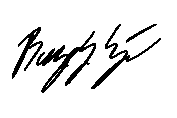
\includegraphics[width=0.3\linewidth]{blank.pdf}
\end{figure}
\begin{flushright}
  \vspace{-1.3cm}
  Boye Gravningen Sjo \\
  Trondhjem, Norge \\
  12th of June 2023
\end{flushright}

\cleardoublepage